\documentclass[10pt]{article}  

%%%%%%%% PREÁMBULO %%%%%%%%%%%%
\title{Reporte de Laboratorio}
\usepackage[spanish]{babel} %Indica que escribiermos en español
\usepackage[utf8]{inputenc} %Indica qué codificación se está usando ISO-8859-1(latin1)  o utf8  
\usepackage{amsmath} % Comandos extras para matemáticas (cajas para ecuaciones,
% etc)
\usepackage{amssymb} % Simbolos matematicos (por lo tanto)
\usepackage{longtable} %agregadom para hacer tablas
\usepackage{xltabular}
\usepackage{tabularray}
\usepackage{graphicx} % Incluir imágenes en LaTeX

\usepackage{color} % Para colorear texto
\definecolor{Blanco}{gray}{1}
\definecolor{Gray}{rgb}{0.501,0.501,0.501}

\usepackage{subfigure} % subfiguras
\usepackage{float} %Podemos usar el especificador [H] en las figuras para que se
% queden donde queramos
\usepackage{capt-of} % Permite usar etiquetas fuera de elementos flotantes
% (etiquetas de figuras)
\usepackage{sidecap} % Para poner el texto de las imágenes al lado
	\sidecaptionvpos{figure}{c} % Para que el texto se alinie al centro vertical
\usepackage{caption} % Para poder quitar numeracion de figuras
\usepackage{commath} % funcionalidades extras para diferenciales, integrales,
% etc (\od, \dif, etc)
\usepackage{cancel} % para cancelar expresiones (\cancelto{0}{x})
 
\usepackage{anysize} 					% Para personalizar el ancho de  los márgenes
\marginsize{2cm}{2cm}{2cm}{2cm} % Izquierda, derecha, arriba, abajo

\usepackage{appendix}
\renewcommand{\appendixname}{Apéndices}
\renewcommand{\appendixtocname}{Apéndices}
\renewcommand{\appendixpagename}{Apéndices} 
% Para que las referencias sean hipervínculos a las figuras o ecuaciones y
% aparezcan en color
\usepackage[colorlinks=true,plainpages=true,citecolor=blue,linkcolor=blue]{hyperref}
%\usepackage{hyperref} 
% Para agregar encabezado y pie de página
\usepackage{fancyhdr} 
\pagestyle{fancy}
\fancyhf{}
\fancyhead[L]{\footnotesize UNI} %encabezado izquierda
\fancyhead[R]{\footnotesize Fac. de Ciencias}   % dereecha
\fancyfoot[R]{\footnotesize Reporte}  % Pie derecha
\fancyfoot[C]{\thepage}  % centro
\fancyfoot[L]{\footnotesize Reporte de conteo y medicion.}  %izquierda
\renewcommand{\footrulewidth}{0.4pt}


\usepackage{listings} % Para usar código fuente
\definecolor{dkgreen}{rgb}{0,0.6,0} % Definimos colores para usar en el código
\definecolor{gray}{rgb}{0.5,0.5,0.5} 
% configuración para el lenguaje que queramos utilizar
\lstset{language=Matlab,
   keywords={break,case,catch,continue,else,elseif,end,for,function,
      global,if,otherwise,persistent,return,switch,try,while},
   basicstyle=\ttfamily,
   keywordstyle=\color{blue},
   commentstyle=\color{red},
   stringstyle=\color{dkgreen},
   numbers=left,
   numberstyle=\tiny\color{gray},
   stepnumber=1,
   numbersep=10pt,
   backgroundcolor=\color{white},
   tabsize=4,
   showspaces=false,
   showstringspaces=false}

\newcommand{\sen}{\operatorname{\sen}}	% Definimos el comando \sen para el seno
%en español

\title{Plantilla para Reportes IMEC-UTB}
% Basada en la plantilla para reportes UPIITA de  Overleaf

%%%%%%%% TERMINA PREÁMBULO %%%%%%%%%%%%

\begin{document}

%%%%%%%%%%%%%%%%%%%%%%%%%%%%%%%%%% PORTADA %%%%%%%%%%%%%%%%%%%%%%%%%%%%%%%%%%%%%%%%%%%%
																					%%%
\begin{center}																		%%%
\newcommand{\HRule}{\rule{\linewidth}{0.5mm}}									%%%\left
 																					%%%

\hspace{0.9cm}

\textsc{\huge Universidad Nacional de Ingeniería }\\[0.8cm]
			
\textsc{\LARGE Facultad de Ciencias}

\vspace{0.6cm}



\includegraphics[scale = 0.15]{Imagenes/UNI.png}

													 								%%%
\vspace*{0.6cm}								%%%
																					%%%	



\begin{minipage}{0.9\textwidth} 
\begin{center}																					%%%
\textsc{\LARGE  Laboratorio de Física BFI01 A\\[0.7cm] Reporte 03}
\end{center}
\end{minipage}\\[0.3cm]
%%%
    																				%%%
 			\vspace*{0.4cm}																		%%%
																					%%%
\HRule \\[0.5cm]																	%%%
{ \huge \bfseries Segunda Ley de Newton}\\[0.2cm]	%%%
 																					%%%
\HRule \\[0.9cm]																	%%%
 																				%%%
																					%%%
\begin{minipage}{0.46\textwidth}													%%%
\begin{flushleft} \large															%%%

% Aqui a continuación pongan los nombres de los integrantes
\emph{El grupo conformado por:}\\[2mm]
Llactahuaman Quispe Benjamin\\20232268G \\[1mm]
Cortez Núñez Christian\\20232203B\\[1mm]
Rocca Cruz Axel\\20234046A\\[1mm]
 

%%%
			%\vspace*{2cm}	
            													%%%
										 						%%%
\end{flushleft}																		%%%
\end{minipage}		
																%%%
\begin{minipage}{0.52\textwidth}		
\vspace{-1.9cm}											%%%
\begin{flushright} \large															%%%
\emph{Profesor:}\\[2mm]																	%%%
Tello Gálvez Julio César\\[1mm]Brocca Pobes Manuel Enrique\\
\end{flushright}																	%%%
\end{minipage}	
\vspace*{1cm}
%\begin{flushleft}
 	
%\end{flushleft}
%%%																	%%%															
\vspace{-2.7cm}	
\begin{flushright}	
\large
\emph{Fecha de la práctica:}\\
\vspace{0.1cm}
3 de mayo de 2023
\end{flushright}
 \vspace{2.4cm}

\large{\today}\\
\vspace{0.3cm}

{ \Large\bfseries 2023-1}
										 			
\end{center}							 											
																					
\newpage																		
%%%%%%%%%%%%%%%%%%%% TERMINA PORTADA %%%%%%%%%%%%%%%%%%%%%%%%%%%%%%%%

\tableofcontents 

\newpage

\begin{center}
    \textbf{\huge Segunda Ley de Newton}
\end{center}

\section{Objetivos}
\subsection{Competencias Generales}
\begin{itemize}
    \item Verificar experimentalmente la segunda ley de Newton
\end{itemize} 
\subsection{Competencias Específicas}
\begin{itemize}
    \item Calibrar dos resortes para hallar su constante elástica y con ello hallar la fuerza que estos aplican sobre un disco.
    \item Hallar la aceleración a partir de los ticks marcados por el disco sobre el papel donde realiza su trayectoria.
\end{itemize}

\section{Datos obtenidos}

\subsection{Calibración de resortes}
\vspace{0,4cm}

\begin{figure}[H]
    \begin{center}
        \caption{Calibración del resorte A}  {\label{fig:A}} 
        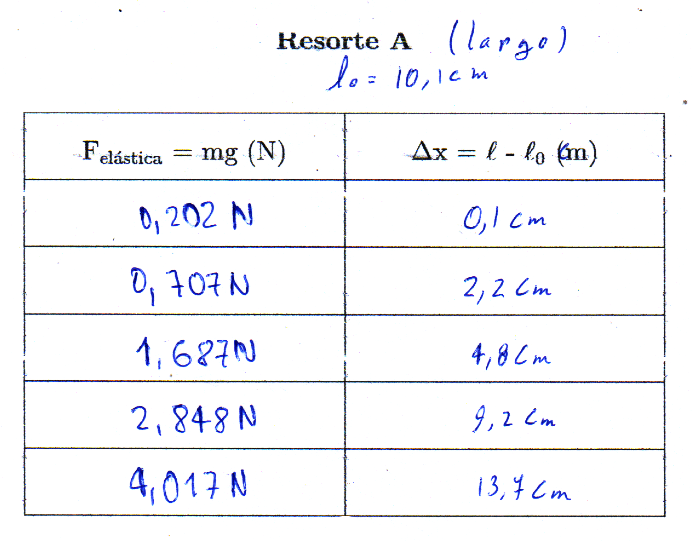
\includegraphics[width = 0.6\textwidth]{Imagenes/ResorteA.png}
    \end{center}
\end{figure}

\begin{figure}[H]
    \begin{center}
        \caption{Calibración del resorte B}  {\label{fig:B}} 
        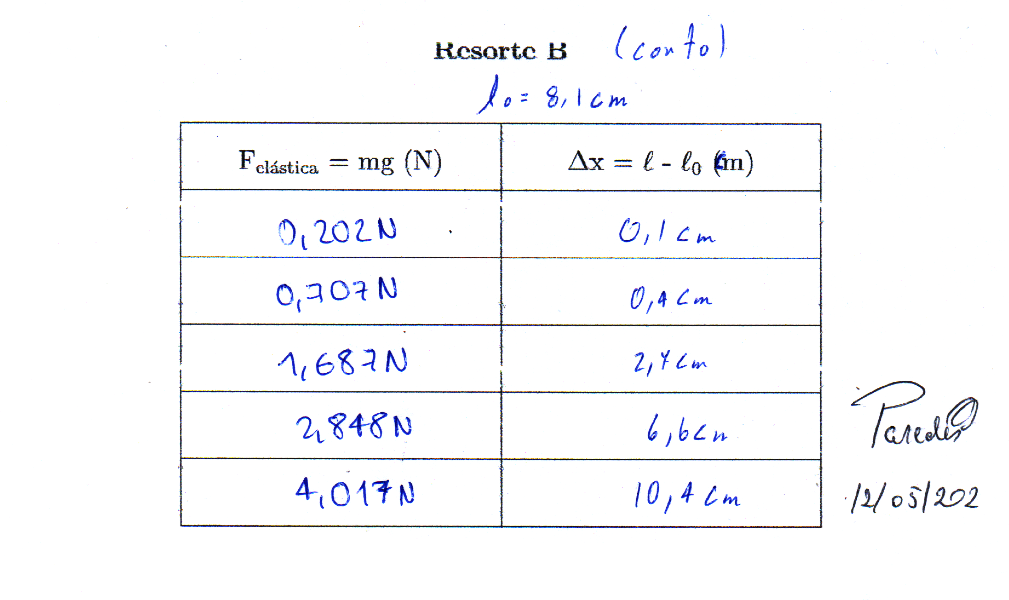
\includegraphics[width = 0.88\textwidth]{Imagenes/ResorteB.png}
    \end{center}
\end{figure}
\vspace{-0,8cm}
\subsection{Módulo de la Fuerza Resultante}

\begin{table}[H]
\caption{Deformación de los resortes y su ángulo formado\\ en 3 puntos de la trayectoria }  {\label{tab:2}}
\centering
\begin{tblr}{
  cells = {c},
  cell{1}{1} = {r=2}{},
  cell{1}{2} = {c=2}{},
  cell{1}{4} = {r=2}{},
  hline{1,6} = {-}{0.1em},
  hline{3} = {-}{},
}
~Punto~ & ~Deformación de cada resorte (m)~ & & ~Ángulos (rad)~ \\
 & ~~~ Resorte A ~~~ & Resorte B &     \\
18      &   0,243  &   0,031     &     1,990           \\
22      &   0,239  &   0,071     &     1,798           \\
25      &   0,203  &   0,093     &     1,955           
\end{tblr}
\end{table}
\vspace{0,5cm}

\subsection{Velocidad y Aceleración instantánea}

\begin{table}[H]
\caption{Distancia de los 3 puntos a sus consecutivos}  {\label{tab:1}}
\centering
\begin{tblr}{
  cells = {c},
  cell{1}{1} = {r=2}{},
  cell{1}{2} = {c=2}{},
  hline{1,6} = {-}{0.1em},
  hline{3} = {-}{},
}
Punto & Distancia al punto consecutivo (m) & \\
      &  ~~~  Anterior ~~~ & Posterior \\
18    & 0,015      & 0,013     \\
22    & 0,009      & 0,011     \\
25    & 0,016      & 0,0175    
\end{tblr}
\end{table}

\newpage

\section{Cálculos y resultados}

\subsection{Curva de calibración y constante elástica de cada resorte}\vspace{2mm}

Uso de los siguientes recursos:    
    \begin{itemize}
        \item Para la Figura \ref{fig:A} y para la Figura \ref{fig:B} definimos:
        \begin{itemize}
            \item y = F$_{el\Acute{a}stica}$
            \item x = $\Delta$x
            \item n = 5 (N° datos)
        \end{itemize}
            
        \item Fórmulas para hallar la ecuación $y = mx + b$ :
    \large{\begin{equation}
        \Bar{x} = \frac{\Sigma x}{n} \textcolor{Blanco}{.............} \Bar{y} = \frac{\Sigma y}{n}
    \end{equation}
    \begin{equation}
        m = \frac{n\Sigma(xy)-(\Sigma x)(\Sigma y)}{n(\Sigma x^{2}) - (\Sigma x)^{2}} 
    \end{equation}
    \begin{equation}
        b = \Bar{y} - m\Bar{x}
    \end{equation}}
\end{itemize}

\subsubsection{Resorte A (0,101 m):}
\vspace{0,2cm}

Formamos la siguiente tabla de datos:

\begin{table}[H]
\centering
\begin{tblr}{
  cells = {c},
  cell{2}{1} = {r=5}{},
  cell{8}{4} = {Gray},
  cell{8}{5} = {Gray},
  cell{8}{6} = {Gray},
  hline{1,9} = {-}{0.1em},
  hline{2,7-8} = {-}{},
}
Variables & x     & y     & xy    & x$^{2}$ & y$^{2}$\\
Datos     & 0,001 & 0,202 & 0,000 & 0,000 & 0,041  \\
          & 0,022 & 0,707 & 0,016 & 0,000 & 0,500  \\
          & 0,048 & 1,687 & 0,081 & 0,002 & 2,846  \\
          & 0,092 & 2,848 & 0,262 & 0,008 & 8,111  \\
          & 0,137 & 4,017 & 0,550 & 0,019 & 16,136 \\
Sumatoria & 0,300 & 9,461 & 0,909 & 0,030 & 27,634 \\
\end{tblr}
\end{table}

\vspace{0,2cm}
Reemplazando en las ecuaciones 1, 2 y 3 obtenemos:

\begin{equation*}
    \Bar{x} = \frac{0,300}{5} = \textbf{0,060} \textcolor{Blanco}{.............} \Bar{y} = \frac{9,461}{5} = \textbf{1,892}
\end{equation*}
\vspace{0,1cm}
\begin{equation*}
    m = \frac{5\times0,909-0,300\times9,461}{5\times0,030 - (0,300)^{2}} = \textbf{28,445} 
\end{equation*}
\vspace{0,1cm}
\begin{equation*}
    b = 1,892 - 28,399\times0,060 = \textbf{0,185}
\end{equation*}\\

\vspace{-0,7cm}
\begin{center}
\textbf{La ecuación de la recta hallada es: $y = 28,445x + 0,185$}\\[0,3cm]
\textbf{La constante elástica del resorte A es: 28,445 N/m}
\end{center}

\newpage

\subsubsection{Resorte B (0,081 m):}
\vspace{0,2cm}

Formamos la siguiente tabla de datos:
\begin{table}[H]
\centering
\begin{tblr}{
  cells = {c},
  cell{2}{1} = {r=5}{},
  cell{8}{4} = {Gray},
  cell{8}{5} = {Gray},
  cell{8}{6} = {Gray},
  hline{1,9} = {-}{0.1em},
  hline{2,7-8} = {-}{},
}
Variables & x     & y     & xy    & x$^{2}$ & y$^{2}$\\
Datos     & 0,001 & 0,202 & 0,000 & 0,000 & 0,041  \\
          & 0,004	& 0,707	& 0,003	& 0,000	& 0,500  \\
          & 0,027 & 1,687	& 0,046	& 0,001	& 2,846  \\
          & 0,066	& 2,856	& 0,188	& 0,004	& 8,157  \\
          & 0,104 & 4,017	& 0,418	& 0,011	& 16,136 \\
Sumatoria & 0,202 &	9,469 & 0,655 & 0,016 &27,680 \\
\end{tblr}
\end{table}

\vspace{0,2cm}
Reemplazando en las ecuaciones 1, 2 y 3 obtenemos:

\begin{equation*}
    \Bar{x} = \frac{0,202}{5} = \textbf{0,040} \textcolor{Blanco}{.............} \Bar{y} = \frac{9,469}{5} = \textbf{1,894}
\end{equation*}
\vspace{0,1cm}
\begin{equation*}
    m = \frac{5\times0,655-0,202\times9,469}{5\times0,016 - (0,202)^{2}} = \textbf{34,756} 
\end{equation*}
\vspace{0,1cm}
\begin{equation*}
    b = 1,894 - 35,102\times0,040 = \textbf{0,503}
\end{equation*}\\

\vspace{-0,7cm}
\begin{center}
\textbf{La ecuación de la recta hallada es: $y = 34,756x + 0,503$}\\[0,3cm]
\textbf{La constante elástica del resorte A es: 34,756 N/m}
\end{center}

\subsection{Módulo de la Fuerza resultante en tres puntos}\vspace{2mm}

Uso de los siguientes recursos:
\begin{itemize}
    \item Datos de la Tabla 1
    \item Ecuaciones de las rectas A y B anteriores
    \item Fórmula de Fuerza Resultante:
    \large{\begin{equation}
        F_{R} = \sqrt{F^{2}_{A} + F^{2}_{B} + 2(F_{A} \times F_{B} \times cos \alpha)}
    \end{equation}}
\end{itemize}

\vspace{0,2cm}
Hallamos las fuerzas F$_{A}$,F$_{B}$ y la F$_{R}$  para cada punto:\\

Punto 18:
 \begin{equation*}
    F_{A} = 28,445 \times (0,243) + 0,185 = 7,097
    \textcolor{Blanco}{--------------}
\end{equation*}
\begin{equation*}
    F_{B} = 34,756 \times (0,031) + 0,503 = 1,580
    \textcolor{Blanco}{--------------}
\end{equation*}  
\begin{equation*}
    F_{R} = \sqrt{(7,089)^{2} + (1,564)^{2} + 2(7,089 \times 1,564 \times cos(1,99)} = \textbf{6,614 N}
\end{equation*}
\vspace{-0,2cm}

Punto 22:
 \begin{equation*}
    F_{A} = 28,445 \times (0,239) + 0,185 = 6,983
    \textcolor{Blanco}{-------------..-}
\end{equation*}
\begin{equation*}
    F_{B} = 34,756 \times (0,071) + 0,503 = 2,971
    \textcolor{Blanco}{--------------}
\end{equation*}  
\begin{equation*}
   \textcolor{Blanco}{..} 
    F_{R} = \sqrt{(6,976)^{2} + (2,968)^{2} + 2(6,976 \times 2,968 \times cos(1,798)} = \textbf{6,947 N}
\end{equation*}

Punto 25:
 \begin{equation*}
    F_{A} = 28,445 \times (0,203) + 0,185 = 5,959 \textcolor{Blanco}{--------------}
\end{equation*}
\begin{equation*}
    F_{B} = 34,756 \times (0,093) + 0,503 = 3,735
    \textcolor{Blanco}{--------------}
\end{equation*}  
\begin{equation*}
    \textcolor{Blanco}{..}
    F_{R} = \sqrt{(5,953)^{2} + (3,740)^{2} + 2(5,953 \times 3,740 \times cos(1,955)} = \textbf{5,726 N}
\end{equation*}
\vspace{-3mm}

\subsection{Velocidad instantánea en los 3 puntos}\vspace{2mm}

Uso de los siguientes recursos
\begin{itemize}
    \item Datos de la Tabla 2
    \item Tiempo entre ticks = 0,025 s
    \item Fórmula:
    \large{\begin{equation}
        V_{i} = \frac{r(P) - r(P-1)}{t~entre~ticks}
    \end{equation}}
\end{itemize}

\vspace{0,2cm}
Hallamos la velocidad entre los instantes intermedios \textbf{anterior} y \textbf{posterior} al punto:\\

Punto 18:
 \begin{equation*}
    V~en~tick = 17,5 \longrightarrow \frac{0,015}{0,025} = \textbf{0,600~m/s}
\end{equation*}
\vspace{0,1cm}
 \begin{equation*}
    V~en~tick = 18,5 \longrightarrow \frac{0,013}{0,025} = \textbf{0,520~m/s}
\end{equation*}

\vspace{0,25cm}
Punto 22:
 \begin{equation*}
    V~en~tick = 21,5 ~ \longrightarrow~ \frac{0,009}{0,025} = \textbf{0,360~m/s}
\end{equation*}
\vspace{0,1cm}
 \begin{equation*}
    V~en~tick = 22,5 ~ \longrightarrow ~ \frac{0,011}{0,025} = \textbf{0,440~m/s}
\end{equation*}

\vspace{0,25cm}
Punto 25:
 \begin{equation*}
    V~en~tick = 24,5 ~ \longrightarrow ~ \frac{0,016}{0,025} = \textbf{0,640~m/s}
\end{equation*}
\vspace{0,1cm}
 \begin{equation*}
    V~en~tick = 24,5 ~ \longrightarrow ~ \frac{0,018}{0,025} = \textbf{0,700~m/s}
\end{equation*}
\vspace{-1mm}

\subsection{Aceleración instantánea en los 3 puntos}\vspace{2mm}

Uso de los siguientes recursos
\begin{itemize}
    \item Datos del cálculo anterior
    \item Tiempo entre ticks = 0,025 s
    \item Fórmula:
    \large{\begin{equation}
        a_{i} = \frac{v(P) - v(P-1)}{t~entre~ticks}
    \end{equation}}
\end{itemize}\vspace{2cm}

Hallamos la aceleración instantánea de los puntos elegidos\\

Punto 18:
 \begin{equation*}
    a = \frac{0,520-0,600}{0,025} = \textbf{-3,200~m/s}^{2}
\end{equation*}
\vspace{0,2cm}

Punto 22:
 \begin{equation*}
    a = \frac{0,440-0,360}{0,025} = \textbf{3,200~m/s}^{2}
\end{equation*}
\vspace{0,2cm}

Punto 25:
 \begin{equation*}
    a = \frac{0,700-0,640}{0,025} = \textbf{2,400~m/s}^{2}
\end{equation*}
\vspace{-1mm}

\subsection{Relación entre Fuerza y Aceleración (F/a)}
\vspace{0,2cm}

Usando los datos de los cálculos anteriores de Fuerza y Aceleración en los 3 puntos, se crea la tabla:

\begin{table}[H]
\centering
\begin{tblr}{
  cells = {c},
  hline{1,5} = {-}{0.08em},
  hline{2} = {-}{},
}
Instante (tick) & \textbar{}a\textbar{} (m/s$^{2}$) & \textbar{}F\textbar{} (N) & \textbar{}$\frac{F}{a}$\textbar{} (Kg) \\
  18  &  3,2  &  6,614  &  2,067  \\
  22  &  3,2  &  6,947  &  2,171  \\
  25  &  2,4  &  5,726  &  2,386  \\
\end{tblr}
\end{table}




\section{Observaciones experimentales}

\section{Cuestionario}
\begin{itemize}
    \item Presente la curva de calibración de cada resorte y calcule la constante elástica de cada resorte
    
    \item Determine en newton el módulo de la fuerza resultante que los resortes ejercieron sobre el disco en 3 puntos de la trayectoria.
    
    \item Determine aproximadamente el vector velocidad instantánea en los instantes intermedios anterior y posterior de los puntos elegidos, es decir si usted eligió el punto correspondiente a t = 8 ticks para hallar la fuerza, halle la velocidad en los instantes t = 7,5 ticks y t = 8,5 ticks. Para ello efectúe la siguiente operación:
    \begin{equation*}
        v(t = 7,5~ticks)= \frac{r(t = 8) - r(t = 7)}{1~tick} 
    \end{equation*}
    
    \item Determine la aceleración instantánea en el punto elegido. Si ese punto es el correspondiente al instante t = 8 tick.
    \begin{equation*}
        a(t = 8~ticks)= \frac{v(t = 8,5) - v(t = 7,5)}{1~tick} 
    \end{equation*}
    
    \item Repita el mismo criterio de los 2 items anteriores sobre los otros dos puntos elegidos.
    \item Determine la relación entre los módulos del vector fuerza y el vector aceleración en cada instante considerado
\end{itemize}

\begin{table}[H]
\centering
\begin{tblr}{
  cells = {c},
  hline{1,5} = {-}{0.08em},
  hline{2} = {-}{},
}
Instante (tick) & \textbar{}a\textbar{} (m/s$^{2}$) & \textbar{}F\textbar{} (N) & \textbar{}$\frac{F}{a}$\textbar{} (Kg) \\
                  &                                &                             &                                \\
                  &                                &                             &                                \\
                  &                                &                             &                                
\end{tblr}
\end{table}


\section{Conclusiones}


\section{Bibliografía}
\begin{itemize}
    \item  Serway. F\'isica. Editorial McGraw-Hill (1992).
    \item Tipler. Física. Editorial Revert\'e (1994).
    \item Taylor, J.R. (2014) Introducci\'on al Análisis de errores - reverte, Taylor 2 Muestra.pdf. Disponible en: https://www.reverte.com/media/reverte/files/book-attachment-3746.pdf (Accessed: April 14, 2023).

\end{itemize}
\end{document}